\section{Validation}

This proposal uses Habanero Java language to describe the implementation details. Using the semantic model for parallel programming languages described in \cite{bouajjani2012analysis}, we can be show that Habanero Java is a superset of other task parallel languages. It contains a wide range of parallel programming constructs that can be used to perform all operations that are possible in other task parallel languages such that Cilk, Chapel, OpenMP3.0, X10 etc. In this section, we describe how to create computation graphs for other task parallel languages. The analysis of these computation graphs proceeds in the same way as analysis of computation graphs for Habanero Java programs. The following examples illustrate the computation graphs for programs written in different task parallel languages.

\begin{enumerate}
\item 
\textbf{X10}
\begin{figure}[H]
\centering
\begin{minipage}[b]{0.35\linewidth}
    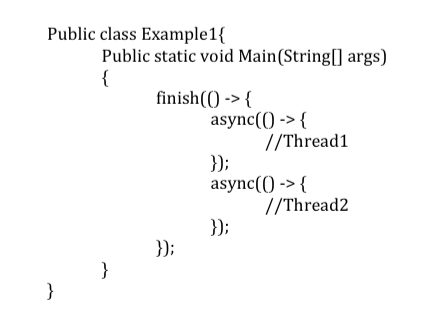
\includegraphics[scale=0.4]{../figs/X10.jpg} 
\caption{X10 Program}
\label{fig:minipage3}
\end{minipage}
\quad
\begin{minipage}[b]{0.35\linewidth}
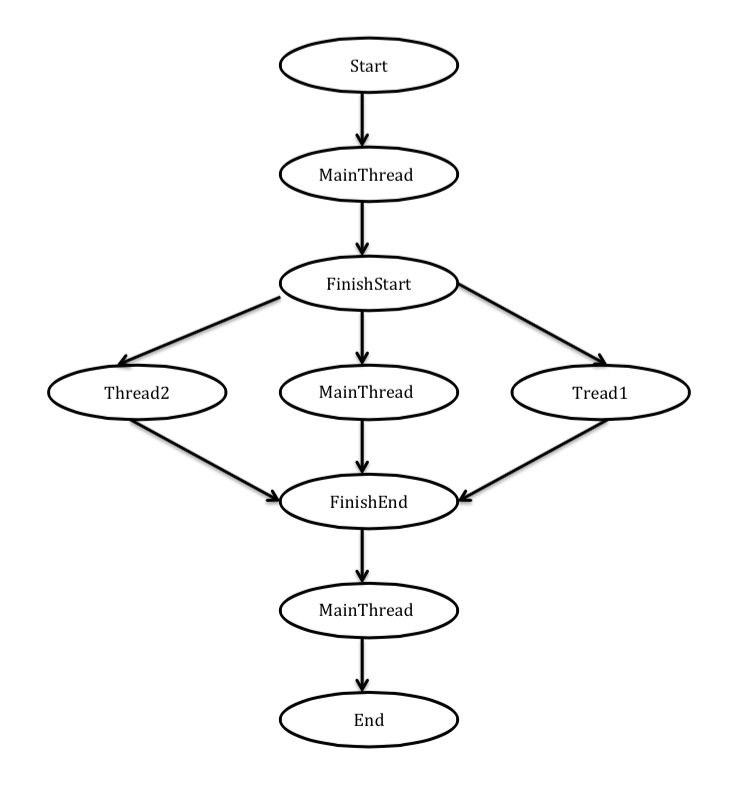
\includegraphics[scale=0.2]{../figs/X10_CG.jpg}
\caption{CG of X10 Program}
\label{fig:minipage4}
\end{minipage}
\end{figure}

\item
\textbf{OpenMP3.0}
\begin{figure}[H]
\centering
\begin{minipage}[b]{0.35\linewidth}
    \includegraphics[scale=0.2]{../figs/Openmp.jpg} 
\caption{Openmp Program}
\label{fig:minipage5}
\end{minipage}
\quad
\begin{minipage}[b]{0.35\linewidth}
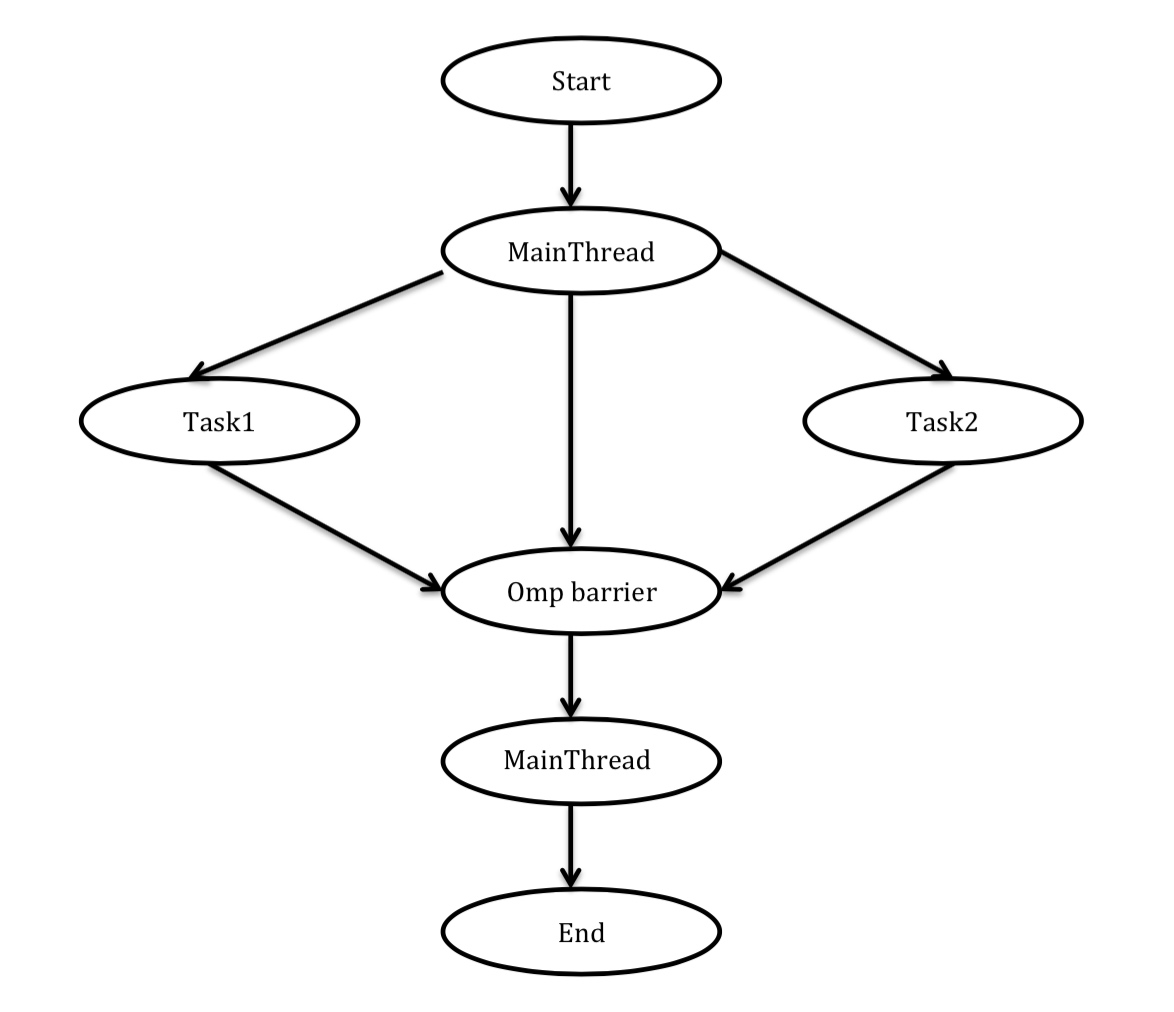
\includegraphics[scale=0.1]{../figs/openmp_CG.jpg}
\caption{CG of Openmp Program}
\label{fig:minipage6}
\end{minipage}
\end{figure}

\item
\textbf{Cilk}
\begin{figure}[H]
\centering
\begin{minipage}[b]{0.35\linewidth}
    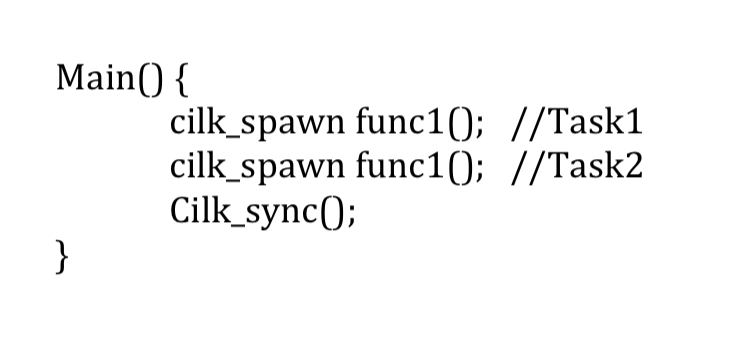
\includegraphics[scale=0.2]{../figs/Cilk.jpg} 
\caption{Cilk Program}
\label{fig:minipage7}
\end{minipage}
\quad
\begin{minipage}[b]{0.35\linewidth}
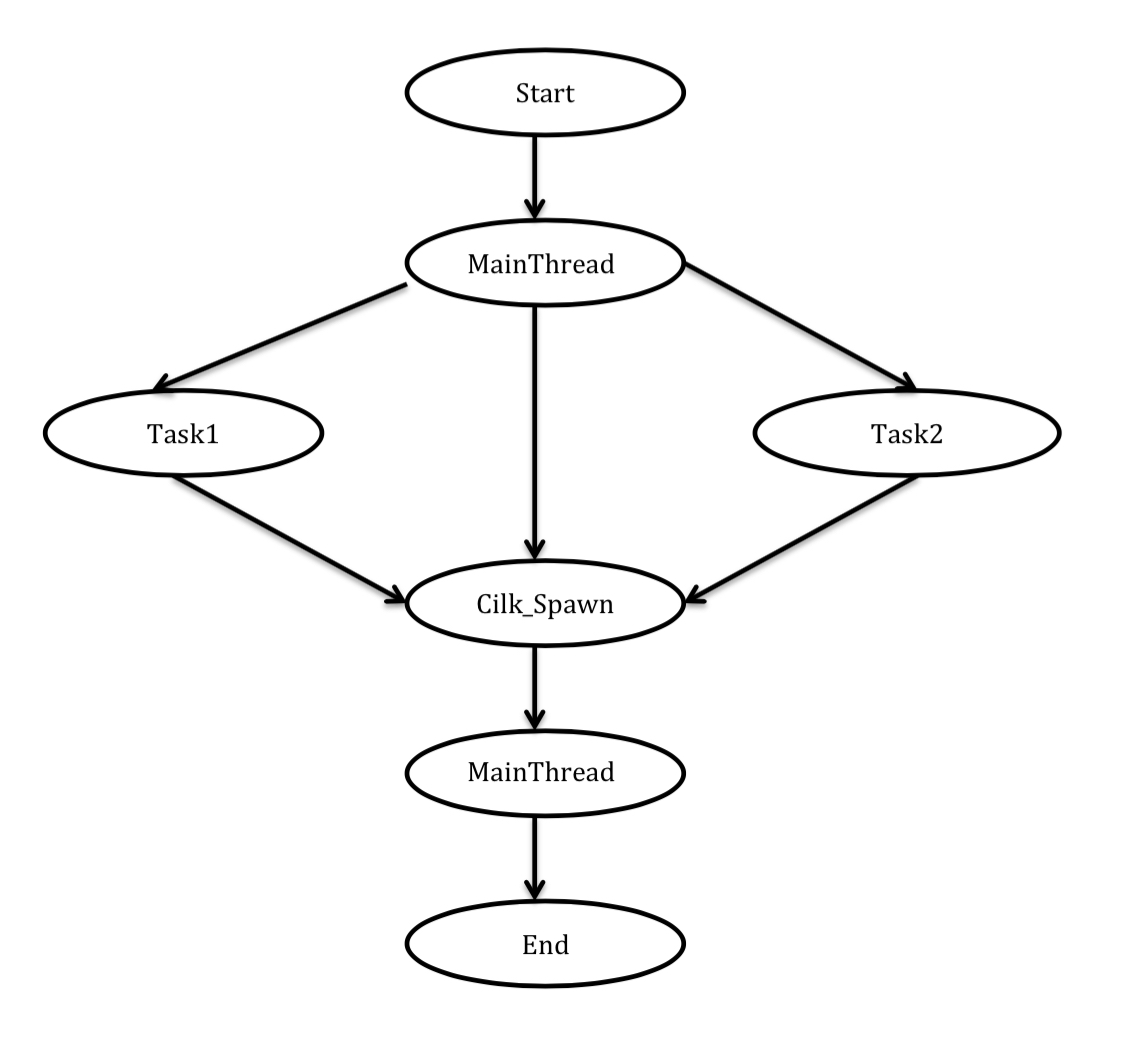
\includegraphics[scale=0.1]{../figs/Cilk_CG.jpg}
\caption{CG of Cilk Program}
\label{fig:minipage8}
\end{minipage}
\end{figure}

\item
\textbf{Chapel}
\begin{figure}[H]
\centering
\begin{minipage}[b]{0.35\linewidth}
    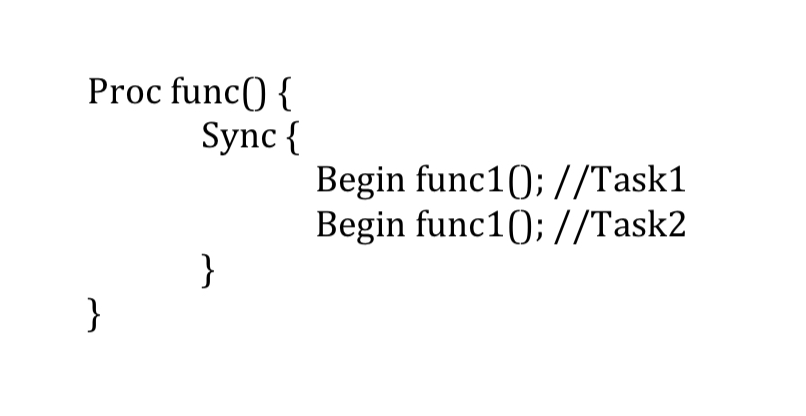
\includegraphics[scale=0.2]{../figs/Chapel.jpg} 
\caption{Chapel Program}
\label{fig:minipage9}
\end{minipage}
\quad
\begin{minipage}[b]{0.35\linewidth}
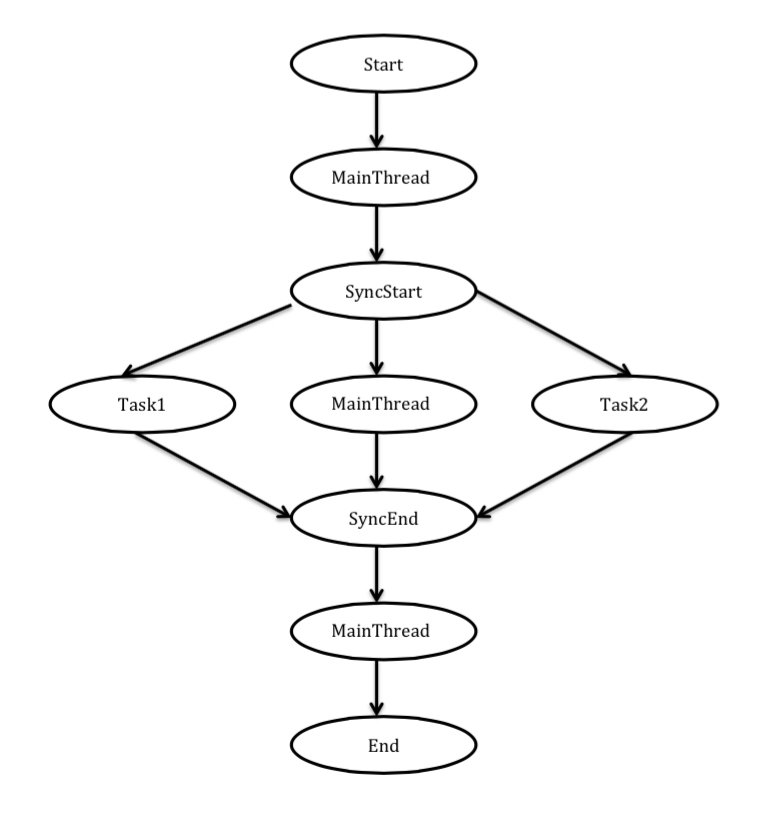
\includegraphics[scale=0.1]{../figs/Chapel_CG.jpg}
\caption{CG of Chapel Program}
\label{fig:minipage10}
\end{minipage}
\end{figure}
\end{enumerate}

To test the correctness of this approach, we have selected benchmarks from the Java Grande Forum benchmarks (JGF) suite, Barcelona OpenMP Task Suites benchmarks (BOTS), Shootout benchmarks suite, and EC2 challenge. The Nqueens and Matrix multiplication benchmarks demonstrate the use of basic parallel programming constructs such as async-finish and loop parallelism constructs such as foreach and forall. The Frannkuch and Mandelbrot benchmarks makes use of the co-ordination construct Isolated in conjunction with the simpler async-finish parallel constructs. The LUFact, SOR and MolDyn benchmarks focus on the co-ordination constructs such as phasers and futures. The BOTS  benchmarks belong to the Barcelona OpenMP Task Suites and focus on various parallel constructs of OpenMP. They have been suitably ported to Habanero Java  to be verified with this tool. The following table lists out the benchmarks that are going to be used for validation. 

\begin{tabular}{|c|c|c|}
\hline
\textbf{Source} & \textbf{Benchmark} & \textbf{Description} \\
\hline
\hline
      & Crypt & IDEA encryption \\
	& LUFact C & LU Factorization \\
  	   & MolDyn & Molecular Dynamics simulation \\
JGF & MonteCarlo & Monte Carlo simulation \\
      & RayTracer & 3D Ray Tracer \\
      & Series & Fourier coefficient analysis \\
      & SOR & Successive over-relaxation \\
      & SparseMatMult & Sparse Matrix multiplication \\
      \hline
      & FFT  & Fast Fourier Transformation \\
	Bots & Health & Simulates a country health system \\
& Nqueens & N Queens problem \\
& Strassen & Matrix Multiply with Strassen’s method \\
\hline
Shootout & Fannkuch & Indexed-access to tiny integer-sequence \\
& Mandelbrot & Generate Mandelbrot set portable bitmap \\
\hline
EC2 & Matmul & Matrix Multiplication \\
\hline
\end{tabular}
\\
\\

In addition to these benchmarks, we are also going to use some micro-benchmarks in Habanero Java that have data races. These 
micro-benchmarks exhibit different deterministic behaviors. These benchmarks are different variations of search algorithm. The following table gives a summary of the tests and their properties. \\

\begin{tabular}{ | c | c | c | c |}
  \hline
  \textbf{Test Case} & \textbf{Data Race Free} & \textbf{Structurally deterministic} & \textbf{Functionally deterministic} \\
  \hline
  Search Count & Y & Y & Y \\
  \hline
  Search & N & Y & Y \\
  \hline
  Search Index & N & Y & N\\
  \hline 
  Search Index With No TaskCreation & N & N & N\\
   after Instance is Found  & & & \\
  \hline 
\end{tabular}